\section{Sea $d(x, y)$ la distancia más corta entre los vértices $x$ y $y$. El diámetro de una
gráfica $G = (V, A)$ se define como $\max{d(x, y) \: \forall x, y \in V (G)}$.}

\subsection{ Diseñar un algoritmo que calcule en tiempo lineal el diámetro de un árbol.
Justificar con sumo detalle la respuesta dada.}


Podemos realizar una búsqueda en profundidad (DFS) desde cualquier vértice $v$ del árbol y
encontrar el vértice $u$ más lejano de $v$. Luego, realizamos otra búsqueda en profundidad desde $u$ 
para encontrar el vértice $w$ más lejano de $u$. El diámetro del árbol será la distancia entre $u$ y
$w$.\\

Para implementar este algoritmo, podemos utilizar una sola función de búsqueda en profundidad. 
La idea es que, durante la búsqueda, mantengamos una variable $maxDist$ que almacene la distancia 
máxima encontrada hasta ese momento, así como otra variable $farthest$ que almacene el vértice más 
lejano del vértice actual. Cada vez que encontremos un vértice que tenga una distancia mayor a 
$maxDist$, actualizamos $maxDist$ y $farthest$.\\

El algoritmo funciona en tiempo lineal ya que realiza dos recorridos en profundidad, 
cada uno de los cuales visita cada vértice del árbol exactamente una vez. 
Por lo tanto, el tiempo de ejecución es $O(n)$, donde $n$ es el número de vértices del árbol.

\subsection{Presentar un árbol de 20 vértices y aplicar el algoritmo}

Arbol Inicial
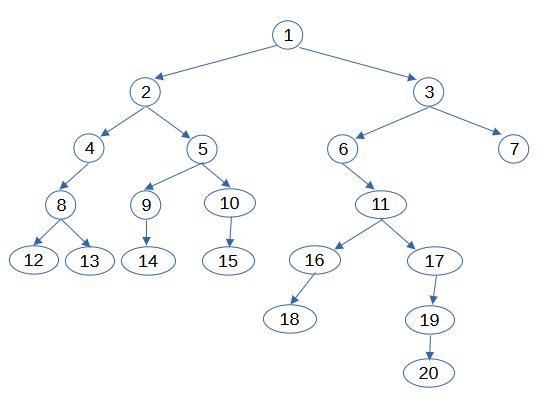
\includegraphics[scale=0.7]{Arbol.png}

Arbol aplicando DFS apartir del vértice inicial \textsc{1}

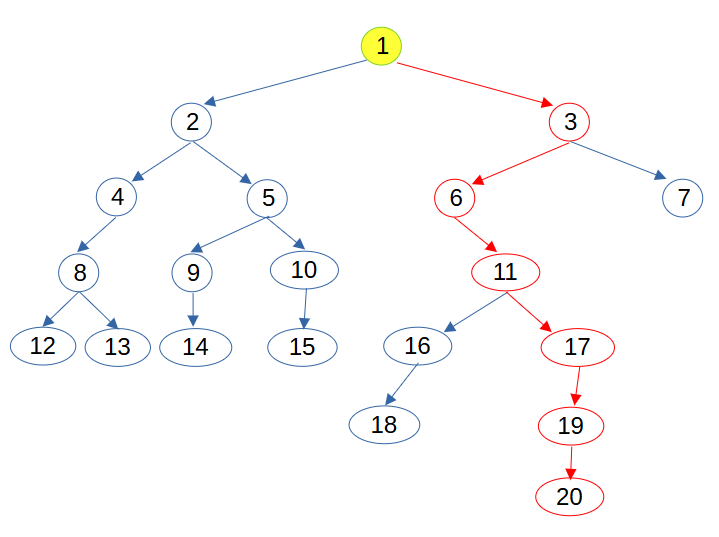
\includegraphics[scale=0.7]{Arbol2.png}

Aqui tenemos 6 pasos.

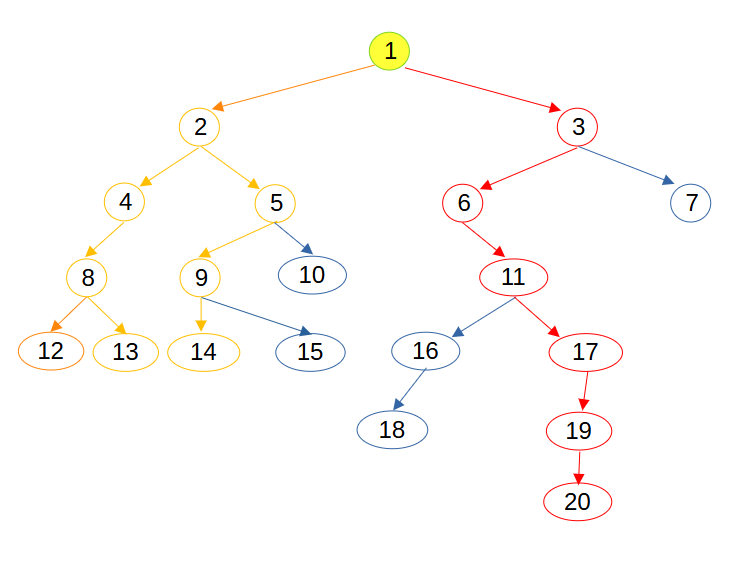
\includegraphics[scale=0.7]{Arbol3.png}

Se aplica DFS desde el vértice 20, 
Como se llega al vértice inicial que fue el primero marcado, se sigue aplicando DFS, así se obtienen 4 niveles más.\\

Por lo tanto el diámetro del árbol es de $6+4=10$
